
\chapter{Utilizzo di GDP - Gathering Detection Platform}\label{UtilizzoDiGDPGatheringDetecionPlatform}

\section{Pagina iniziale}\label{UtilizzoDiGDPGatheringDetecionPlatformPaginaIniziale}
La pagina iniziale che si presenta all'avvio è mostrata nella seguente figura.
Al suo interno troviamo il nome della web application$_{\scaleto{G}{3pt}}$ seguito dalle componenti qui elencate e successivamente spiegate:
\begin{enumerate}
	\item La barra di navigazione;
	\item Contenuto centrale;
	\item Il footer.
\end{enumerate}

\begin{center}
	\begin{figure}[H]
		\centering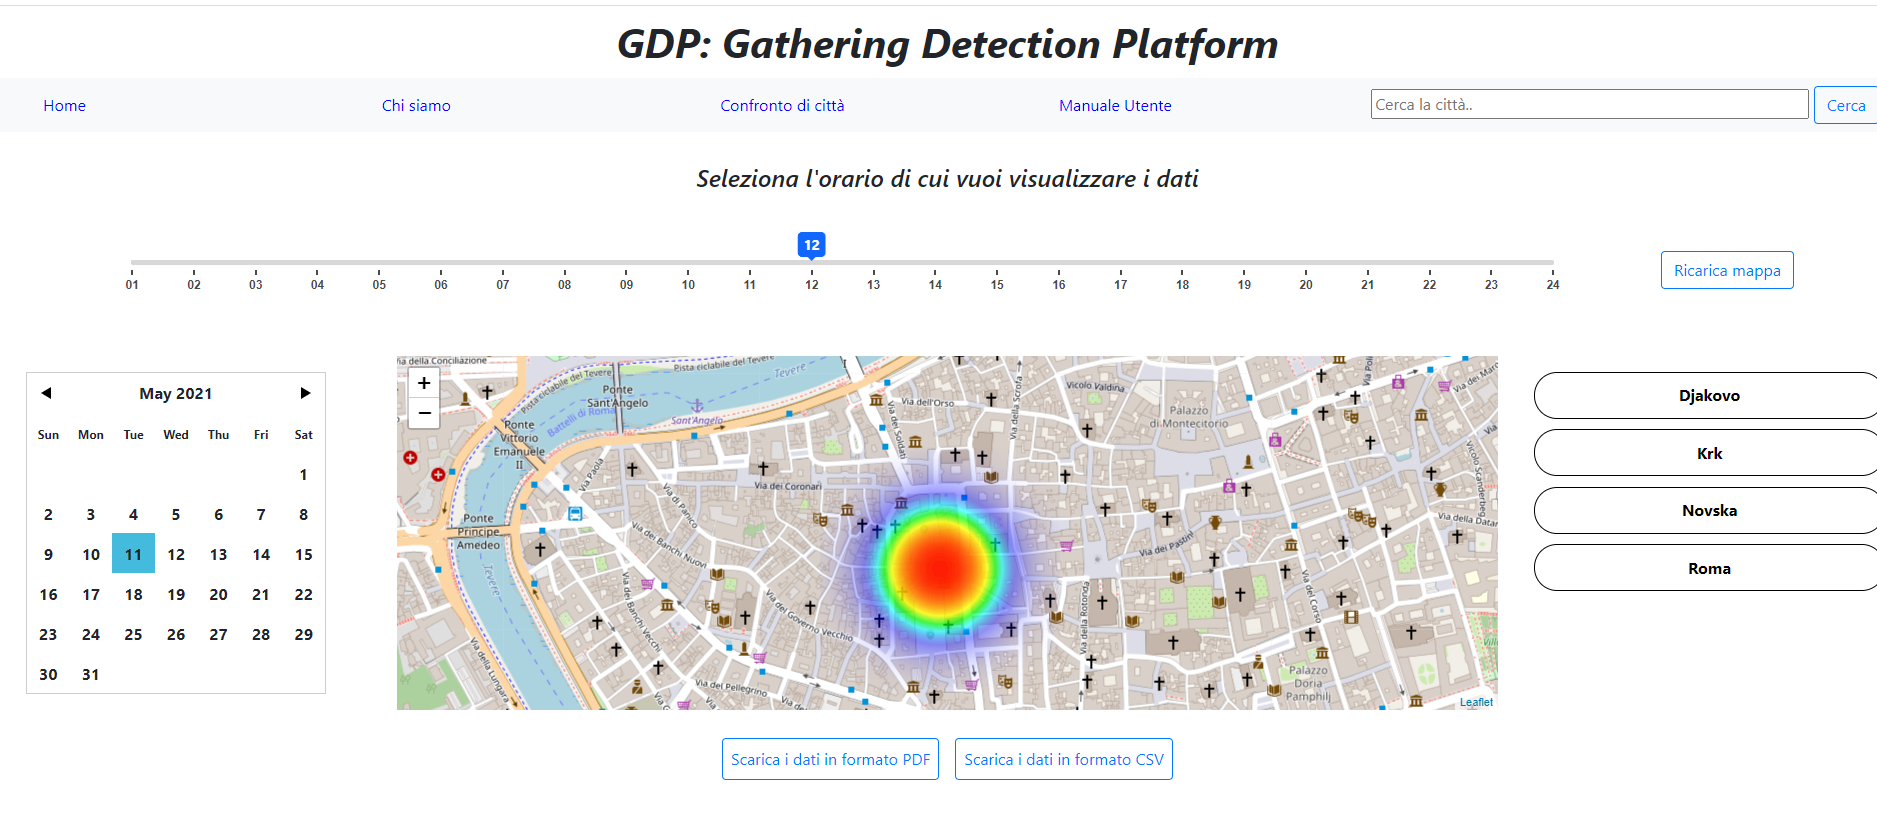
\includegraphics[width=0.9\linewidth]{../immagini/manualeUtente/heatmapsenzapopup.png}
		\caption{\textbf{\textbf{\textbf{Pagina iniziale}}}}
	\end{figure}
\end{center}

\section{Barra di navigazione}\label{UtilizzoDiGDPGatheringDetecionPlatformBarraDiNavigazione}

La barra di navigazione dell'applicazione web$_{\scaleto{G}{3pt}}$ è quella rappresentata in figura 3.2. Tramite questa l'utente potrà navigare all'interno della piattaforma. Nella barra di navigazione sono presenti:
\begin{enumerate}
	\item \textit{Home}: link alla pagina iniziale;
	\item \textit{Chi siamo}: link alla pagina "Chi siamo";
	\item \textit{Confronto città}: link alla pagina in cui si può effettuare il confronto del flusso di persone fra due città.
	\item \textit{Manuale d'uso}: link per scaricare in formato pdf il manuale d'uso, in modo da conoscere tutte le funzionalità offerte dalla web-app$_G$ ed il loro funzionamento;
	\item \textit{Barra di ricerca}: attraverso la barra di ricerca è possibile cercare, e quindi selezionare tra quelle disponibili, la città di cui si è interessati a visualizzare i dati sulla heat-map$_G$. La ricerca può avvenire sia in base al nome della città sia in base al codice numerico della webcam associata ad ogni città. \\
	Per il codice numerico l'associazione città-codice attualemte è la seguente:
	\begin{itemize}
		\item id{\_}webcam = 1, città = Roma;
		\item id{\_}webcam = 2, città = Novska;
		\item id{\_}webcam = 3, città = Djakovo;
		\item id{\_}webcam = 4, città = Krk.
	\end{itemize}
	\textit{Nel caso in cui vengano aggiunte città nel database, verrà aggiornato tale elenco che associa il codice alla città. Analogamente verrà aggiornato il manuale d'uso reperibile dalla web-app$_G$} \\
	Infine, se la città o il codice ricercato non è presente nel database, verrà visualizzato un messaggio d'errore che informa l'utente di ciò.
\end{enumerate}

\begin{center}
	\begin{figure}[H]
		
\includegraphics[width=1\linewidth]{../immagini/manualeUtente/navbar.png}
		\caption{\textbf{Barra di Navigazione}}
	\end{figure}
\end{center}

\section{Contenuto centrale}\label{UtilizzoDiGDPGatheringDetecionPlatformContenutoCentrale}

\subsection{Pagina Iniziale - Home} \label{UtilizzoDiGDPGatheringDetecionPlatformContenutoCentralePaginaInizialeHome}
La pagina iniziale che visualizza l'utente è quella mostrata in figura 3.1.

\subsubsection{Heatmap}\label{UtilizzoDiGDPGatheringDetecionPlatformContenutoCentralePaginaInizialeHomeHeatmap}
Al centro della web app$_{\scaleto{G}{3pt}}$ è presente una heat map$_{\scaleto{G}{3pt}}$ che raffigura, inizialmente, il flusso di persone presenti nella città di Roma nell'orario attuale. Successivamente l'utente potrà modificare la città, attraverso l'elenco delle città (\S~\ref{UtilizzoDiGDPGatheringDetecionPlatformContenutoCentralePaginaInizialeHomeMenùATendina}) oppure tramite la barra di ricerca, l'orario e la data, secondo quanto spiegato in \S~\ref{UtilizzoDiGDPGatheringDetecionPlatformContenutoCentralePaginaInizialeHomeCalendarioESlider}, e visualizzare tramite la heat map$_{\scaleto{G}{3pt}}$ i dati relativi ai campi selezionati. Inoltre, l'utente ha anche la possibilità di modificare lo zoom della mappa, effettuando lo zoom-in o lo zoom-out di questa. \\
Per facilitare la lettura della mappa, dopo che l'utente ha effettuato lo zoom-in, viene mostrato un pop-up, accompagnato da un marker, che evidenzia sia il nome del luogo che si sta osservando sia il numero di persone effettivamente presenti in quel momento. Il messaggio nel pop-up, in aggiunta, informa l'utente sul tipo di dato che sta visualizzando, ovvero se i dati in questione sono reali o predetti, scrivendo fra parentesi la tipologia. \\
L'utente ha la possibilità di chiudere il pop-up. Questa funzionalità viene illustrata nella figura successiva.

\begin{center}
	\begin{figure}[H]
		\centering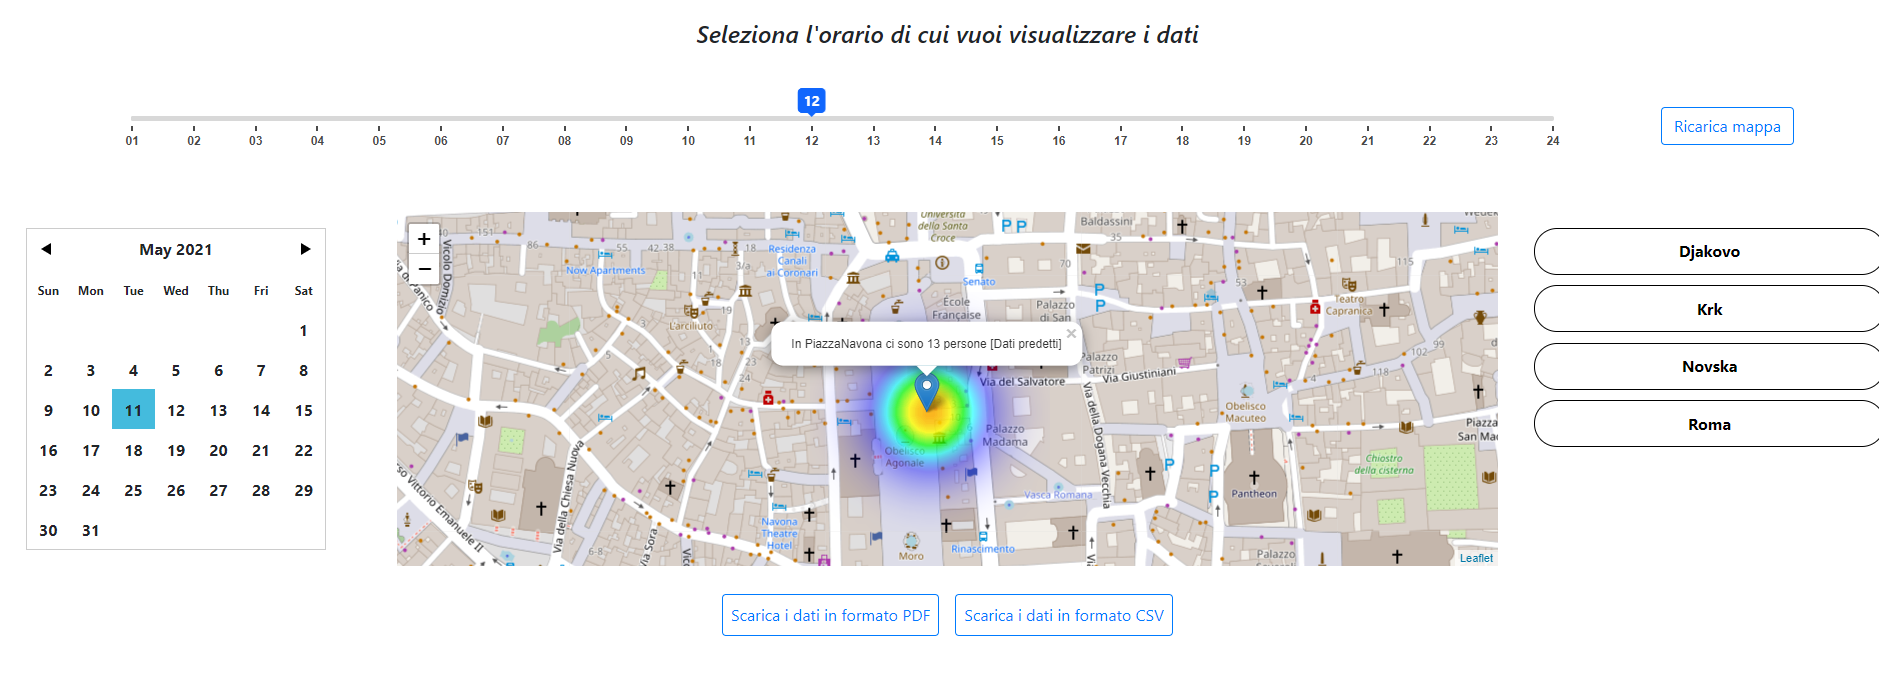
\includegraphics[width=0.9\linewidth]{../immagini/manualeUtente/heatmapPopup.png}
		\caption{\textbf{\textbf{\textbf{Heatmap con popup visibile}}}}
	\end{figure}
\end{center}

\subsubsection{Elenco delle città} \label{UtilizzoDiGDPGatheringDetecionPlatformContenutoCentralePaginaInizialeHomeMenùATendina}
L'elenco delle città, posizionato a destra della mappa, viene utilizzato per la selezione della città. Infatti, l'utente, quando apre l'applicazione web$_{\scaleto{G}{3pt}}$, visualizza la mappa centrata sulla città di Roma, la città di default, ma successivamente può scegliere di osservare il flusso di persone relativo ad un'altra città presente tra quelle messe a disposizione nella lista.


\subsubsection{Calendario e slider}\label{UtilizzoDiGDPGatheringDetecionPlatformContenutoCentralePaginaInizialeHomeCalendarioESlider}
L'utente ha a disposizione, a sinistra della mappa, un calendario che gli permette di scegliere l'anno, il mese ed il giorno di cui desidera visualizzare i dati. Per selezionare il mese bisogna spostarsi usando le frecce poste ai lati (1), mentre per l'anno si seleziona sull'anno corrente (2).
\begin{center}
	\begin{figure}[H]
		\centering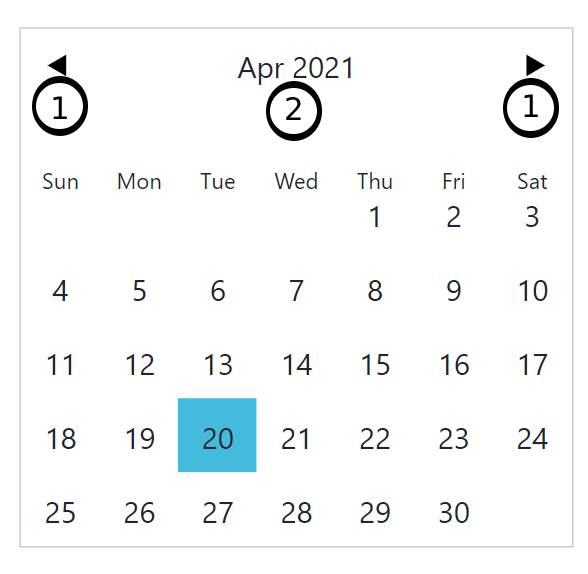
\includegraphics[width=0.3\linewidth]{../immagini/manualeUtente/Calendario.jpg}
		\caption{\textbf{Calendario}}
	\end{figure}
\end{center}
Al di sopra della mappa, invece, è presente uno slider$_G$ con il quale l'utente può scegliere un orario diverso da quello attuale di cui desidera visualizzare i dati attraverso la heat map$_{\scaleto{G}{3pt}}$. La selezione dell'orario è effettuata su intervalli di tempo di ora in ora. Per selezionare l'ora attravero lo slider$_{\scaleto{G}{3pt}}$, si può sia cliccare sulla scritta dell'orario che si vuole selezionare sia spostare l'etichetta rappresentante l'ora selezionata(1).
\begin{center}
	\begin{figure}[H]
		\centering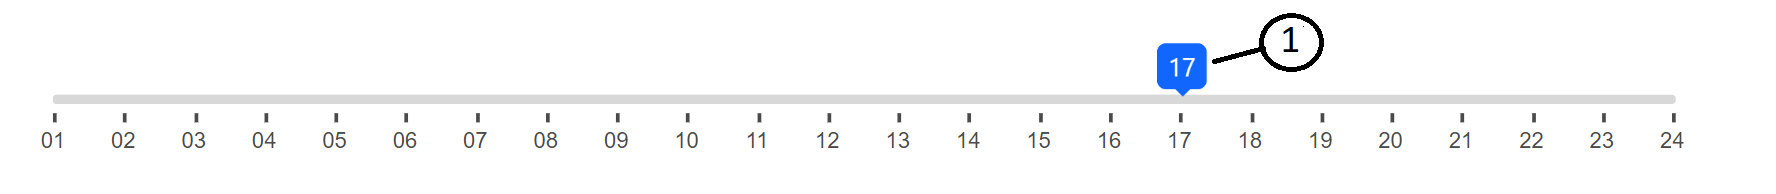
\includegraphics[width=1\linewidth]{../immagini/manualeUtente/Slider.png}
		\caption{\textbf{Slider}}
	\end{figure}
\end{center}

\subsubsection{Bottone Reload Map} \label{UtilizzoDiGDPGatheringDetecionPlatformContenutoCentralePaginaInizialeHomeBottoneReloadMap}
Nel caso in cui l'utente avesse selezionato una data diversa da quella odierna e/o un'ora differente da quella attuale, cliccando sul pulsante "Reload Map", la mappa si aggiornerà e tornerà a mostrare i dati in tempo reale, quindi relativi a data e ora corrente, rimanendo sulla città che si stava osservando.
\begin{center}
	\begin{figure}[H]
		\centering
\includegraphics[width=0.3\linewidth]{../immagini/manualeUtente/ReloadMap.png}
		\caption{\textbf{Reload Map}}
	\end{figure}
\end{center}

\subsubsection{Bottoni Download dati} \label{UtilizzoDiGDPGatheringDetecionPlatformContenutoCentralePaginaInizialeHomeBottoneDownloadDati}
\paragraph{Download dati pdf}
Il bottone Download dati PDF permette all'utente di scaricare, in formato pdf, tutti i dati storicizzati nel database relativi alla città che si sta osservando.

\paragraph{Download dati csv}
Il bottone Download dati csv permette all'utente di scaricare, in formato csv, tutti i dati storicizzati nel database relativi alla città che si sta osservando.

\subsubsection{Messaggio d'errore} \label{UtilizzoDiGDPGatheringDetecionPlatformContenutoCentralePaginaInizialeHomeMessaggioDiErrore}
Nel caso in cui non ci siano dati disponibili nel database per il luogo, il giorno e l'ora in questione, l'utente visualizzerà un messaggio di errore che lo informerà del disguido e la mappa non mostrerà nessun dato. L'utente potrà chiudere il messaggio d'errore premendo il pulsante "OK".


\subsection{Chi siamo} \label{UtilizzoDiGDPGatheringDetecionPlatformContenutoCentraleChiSiamo}
In questa pagina è possibile visualizzare le informazioni che riguardano il team di sviluppo \textit{Jawa Druids}, l'azienda proponente \textit{Sync Lab} e il progetto \textit{GDP: Gathering Detection Platform}.


\subsection{Confronto città} \label{UtilizzoDiGDPGatheringDetecionPlatformContenutoCentralePaginaInizialeHomeBottoneConfrontoCitta}
In questa pagina l'utente ha la possibilità di confrontare il flusso di persone di due città. L'utente, infatti, deve selezionare, tramite i due appositi pulsanti, le due città, tra quelle presenti nel database, di cui desidera avere il confronto. \\
 Premuto il pulsante "Confronta", apparirà sullo schermo una frase che riassume quante persone sono presenti nelle due città selezionate. \\
 Se l'utente non specifica diversamente, egli vedrà il confronto dei dati delle due città in real time, ovvero del giorno e dell'ora attuali. Come nel caso della visualizzazione su heat-map, c'è la possibilità, per l'appunto, di selezionare un giorno ed un orario differenti da quelli correnti e di visualizzare quindi il confronto fra le due città relativo alle impostazioni scelte. \\
 Nel caso in cui l'utente non abbia selezionato una od entrambe le città, o se non ci sono dati disponibili nel database per le città, l'ora o il giorno scelto, verrà visualizzato un messaggio d'errore che informerà l'utente di tale problema (si veda \S~\ref{UtilizzoDiGDPGatheringDetecionPlatformContenutoCentralePaginaInizialeHomeMessaggioDiErrore} per maggiorni informazioni).

\section{Footer}\label{UtilizzoDiGDPGatheringDetecionPlatformFooter}
Il footer è presente in tutte le pagine dell'applicazione web$_{\scaleto{G}{3pt}}$ e riporta alcuni link utili, come quello del sito web dell'azienda \textit{Sync Lab} e la mail del team di sviluppo, da contattare in caso si riscontrino problemi con l'uso del prodotto software$_{\scaleto{G}{3pt}}$.
%da sistemare
